\section{Windows Credential Management}
\paragraph{Logon Session}
User Credentials are stored in lsass.exe (OS might use them later to SSO to other services).
User Credentials are tied to \textbf{authentication packages} inside of the logon session, e.g.:
\begin{itemize}
  \item NTLM hashes
  \item Kerberos tickets/keys
  \item Passwords in plaintext
\end{itemize}

\paragraph{Tokens}
Current security context of a process/thread:
\begin{itemize}
  \item If a thread/process wants to act in the name of a user, it uses a token
  \item Tokens are tied to a logon session and determine how the cred is used
\end{itemize}

\subsection{Logon Sessions}
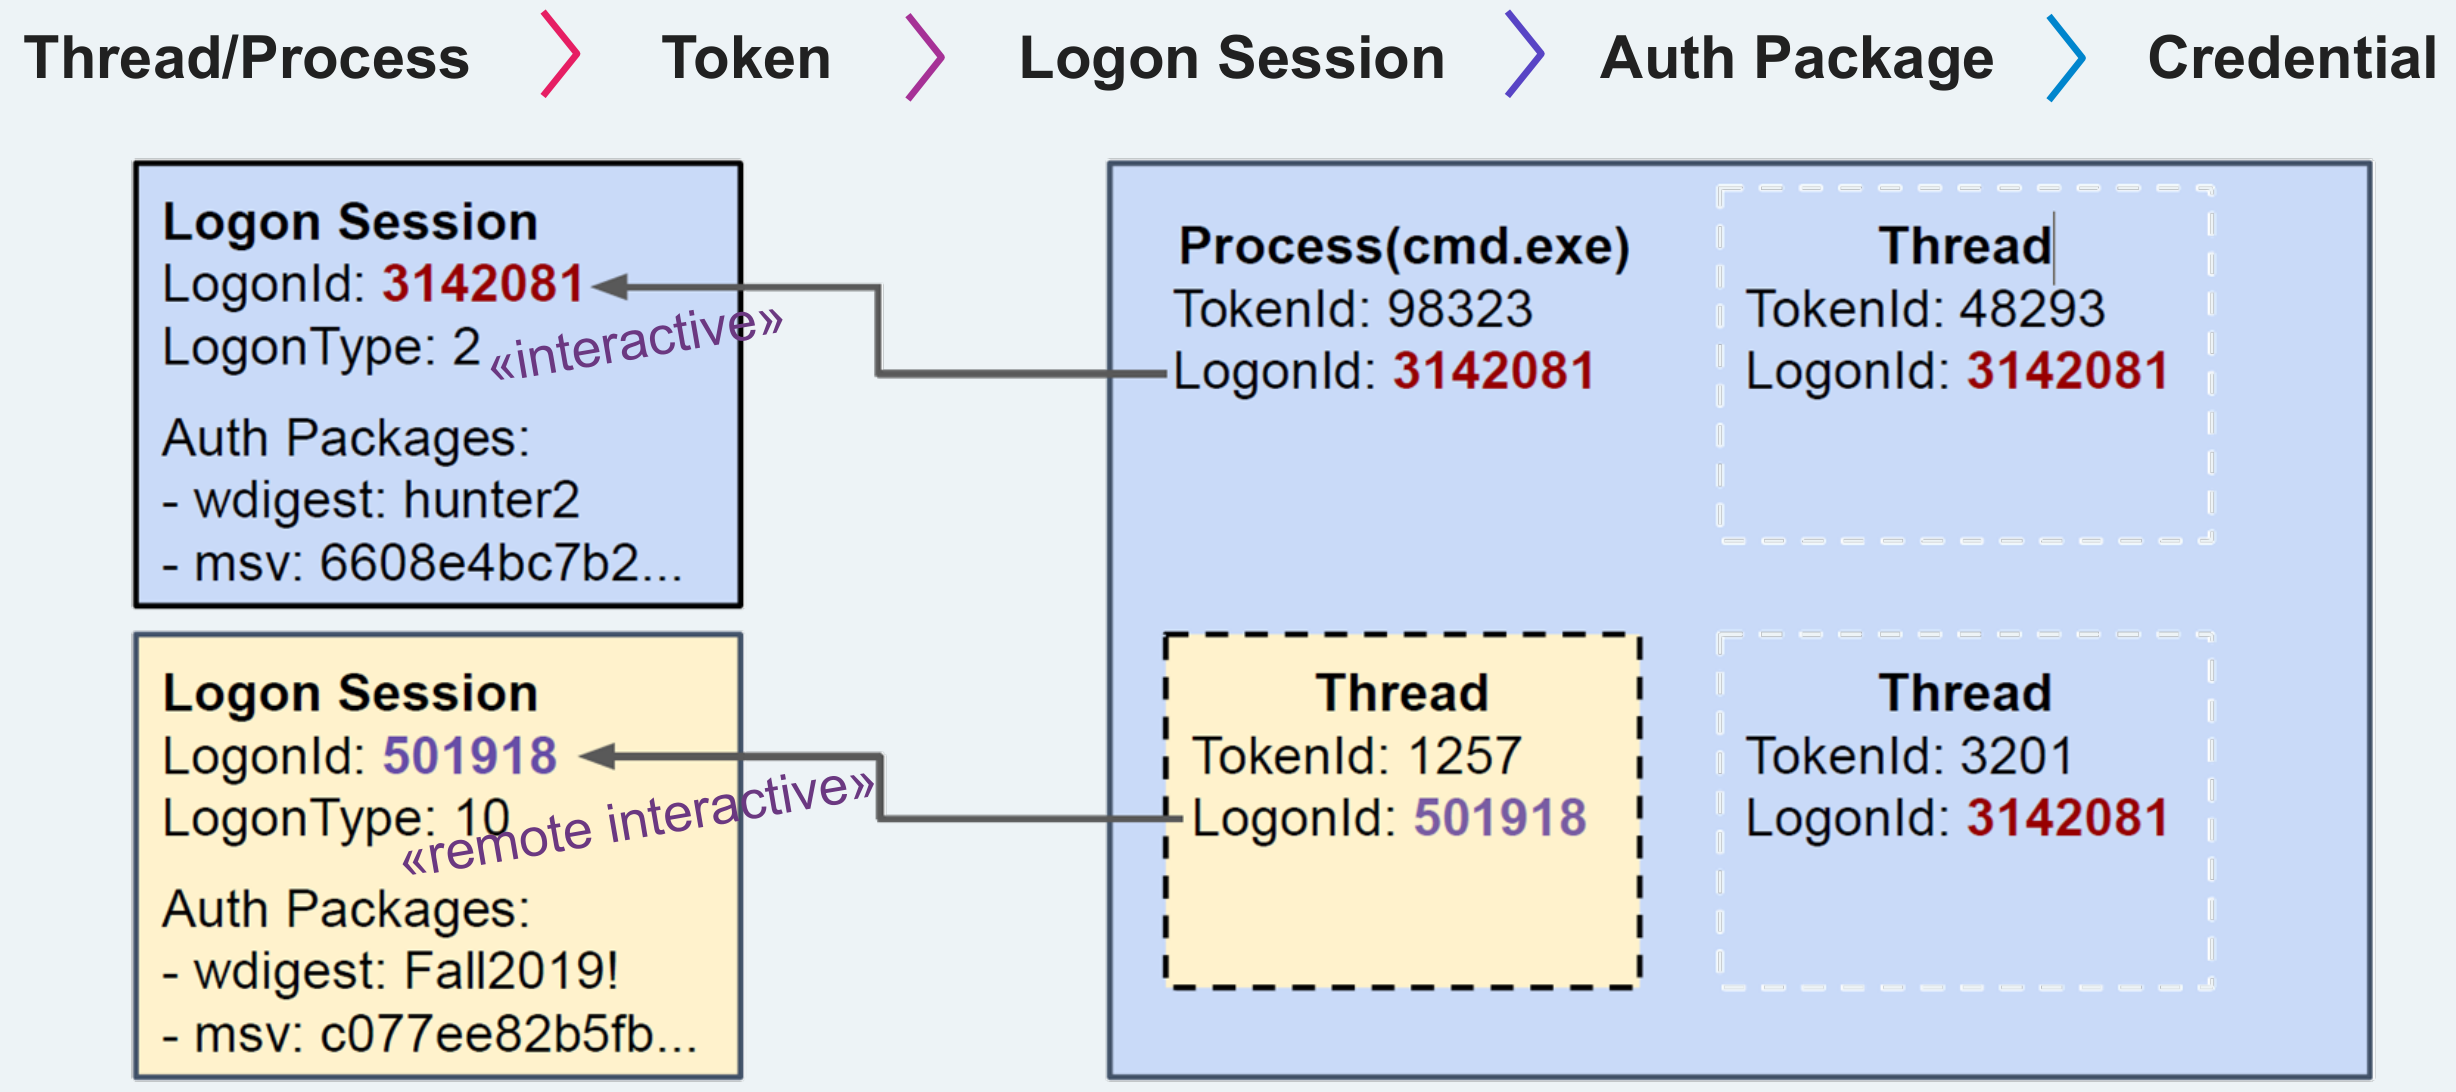
\includegraphics[width=\linewidth]{logon-session.png}

\subsubsection{Credential Theft}
Important Logon Types to understand:
\begin{itemize}
  \item \textbf{Network Logons} (Type 3) - clients prove they have the credentials but do not send them
  \item \textbf{Non-Network Logons} (Interactive/NetworkCleartext/\dots) - credentials are sent to the server and therefore stored in LSASS memory
\end{itemize}

\subsubsection{The ``Double-Hop Problem''}
When you remotely execute code with WMI or WinRM, you'll receive a token that is tied to a Network Logon session, meaning the credentials are not actually sent to the remote host. This means that you can't ``double-hop'' and authenticate to other resources in the network from this compromised host!

\paragraph{Work Arounds}
Use another token that points to a non-network logon session, either by:
\begin{itemize}
  \item stealing a token
  \item injecting into another process
\end{itemize}
Create a new token that points to a non-network logon session using stolen credentials:
\begin{itemize}
  \item make\_token [DOMAIN/user] [password]
  \item spawns [DOMAIN/user] [password] [listener]
  \item pth [DOMAIN/user] [HASH]
\end{itemize}

\subsection{Tokens}
\begin{itemize}
  \item \textbf{Primary Tokens}: a process token. The security context is the user associated with the process.
  \item \textbf{Impersonation Tokens}: a thread token. Used to impersonate other tokens in client/server scenarios. Depending on impersonation level the OS might use the tokens creds to authenticate remotely.
\end{itemize}
\paragraph{Impersonation Levels}
\begin{itemize}
  \item \textbf{Anonymous}: Remote Server can't identify a client, the thread acts as an anonymous user
  \item \textbf{Identification}: Remote server can identify user, but not impersonate
  \item \textbf{Impersonation}: The remote server can identify and impersonate the client across one computer boundary (Network Logon to the server)
  \item \textbf{Delegation}: The server can impersonate the client across multiple boundaries, and can make calls on behalf of the client (known as Kerberos ``double hop'')
\end{itemize}
If you steal an Impersonation Token with Anonymous or Identification Impersonation Level, remote authentication will fail!\\

If you steal a Process Token or an Impersonation Token with Impersonation or Delegation Level, remote authentication might work! (if the corresponding logon session has credentials in it)

\subsubsection{With Mimikatz}
Mimikatz can interact with process and thread tokens. The token:: module enables to interact with authentication tokens, including grabbing and impersonating existing tokens.
\begin{lstlisting}
  #list all tokens of the system
  token::list 

  #impersonate a token
  token::elevate /id:<tokenId>
\end{lstlisting}

\subsubsection{With Cobalt Strike}
Cobalt Strike can only steal process tokens:
\begin{lstlisting}
  #command will impersonate the token of the given process ID, granted you have rights to impersonate
  steal_token <PID>

  #will revert back to your normal token security context
  rev2self
\end{lstlisting}
Cobalt Strike can also create new logon sessions and point token to that:
\begin{lstlisting}
  #Creates a new logon session using stolen credentials
  make_token <DOMAIN\user> <password>
\end{lstlisting}